\subsection{Architectual Design}
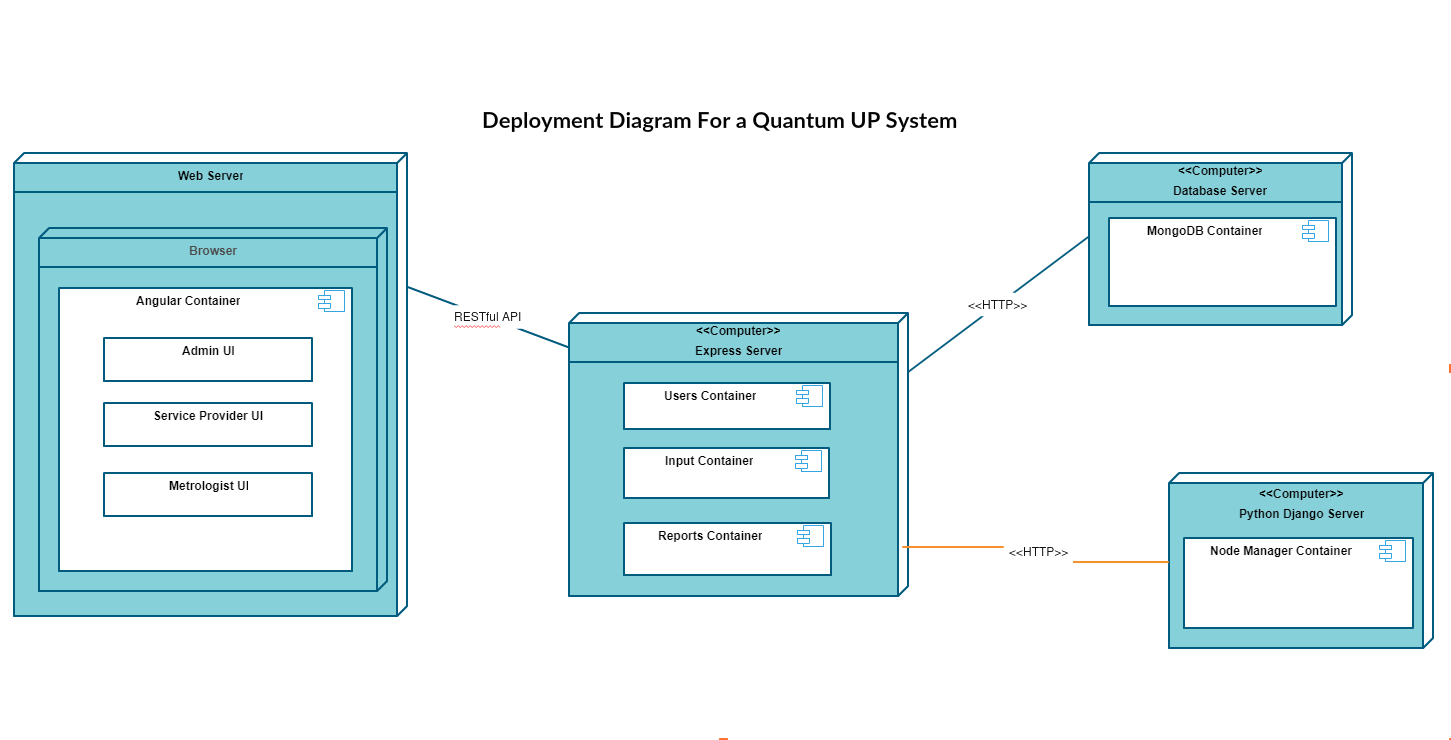
\includegraphics[width=\textwidth]{deployment_diagram/Quantum_UP_Deployment_Diagram.png}
    \begin{center}
    	\small{Figure 32: Deployment Diagram for Quantum UP System}
    \end{center}

For the architectural design we went with micro services because micro services promotes \textbf{low coupling} by making each component run only their services that is required by it. The main way that this will be done is to use docker where each \textbf{docker} container will communicate with each other via HTTP and ports. By using docker it makes each container very secure and also promotes \textbf{portability} where on any server the relevant docker containers can be run and linked. This makes it very easy to move your system without having to spend time installing dependencies and make sure everything is installed before running the system. The GUI services will be provided by an \textbf{Angular} app because angular make binding and usage very simple which aids in user experience. The Angular app will make API calls to a dockerized express server which will hold the user,input and reporting services. When a request is made to the relevant service.\\ \\ 

The service will either make a request to store data on the dockerized \textbf{MongoDB} database server or it will make a request to the node manager container that will run the nodes services for benchmarking. The reason to use MongoDB as the server is because it is lightweight and allows for rapid scaling on large amounts of data, which might be the case in this situation. Another good thing about micro services is that each service does not have to know what the other service is doing and does not have to rely on other services thus making it very \textbf{modular}. If you would not want to depend on a local Db or just one DB, the ease of micro services allows you to switch out database with minimal changes. For example switching out MongoDb for a cloud database such as Cosmos Db with a Mongo API so there is no need to change database write commands.\\ \\

Finally the node manager that will run the benchmarking services will run in a python Django server. The reason for using python is that it works well with getting low level data like CPU usage which is useful in this case and since micro services are used it allows for language neutral communication because data is communicated via HTTP and API calls.Theses reasons above are why a micro services architecture would be good for this system.

\subsection{Technologies used( refer above for description of how theses technologies are used)}
\begin{itemize}
    \item Docker        - To containerize services
    \item Express JS    - Server
    \item Nodejs        - Server language
    \item Angular 5     - Live Binding, Very responsive UI
    \item MongoDB       - Database
    \item Django        - Python Server
\end{itemize}